\documentclass[9pt,onecolumn,twoside]{pnas-new}
% Remove the twocolumn option to create a single column SI file if required. 
% Use the lineno option to display guide line numbers if required.
% Note that the use of elements such as single-column equations
% may affect the guide line number alignment. 

\templatetype{pnassupportinginfo}

\title{Supporting Information}
\author{Hough et al.}

\doi{genetics.XXXXXXXXXX}

\begin{document}

\maketitle

\section*{Supporting Information (SI)}

All supporting information can be obtained from https://github.com/houghjosh/XYdiversity.

\section*{SI Tables}

\begin{table}[tbhp!]
\centering
\caption{Population identities (ID) and location information for \textit{R. hastatulus} samples from Texas and North Carolina}
\begin{tabular}{lllll}
Population ID & Location & Altitude & Latitude & Longitude \\
\midrule
\textbf{Texas} &  &  &  &  \\
TX-MTP & Mount Pleasant, Texas & 130	 & 33.17453 & 94.98799 \\
OK-RAT & Rattan, Oklahoma & 138 & 34.15755 & 95.41325 \\
TX-LIV & Livingston, Texas & 83 & 30.69947 & 94.79981 \\ 
LA-DER & De Ridder, Lousiana & 67 & 30.8941 & 93.3143 \\
TX-ATH & Athens, Texas & 145 & 32.18471 & 95.8032 \\
OK-WIL & Willis, Oklahoma & 211 & 33.89663 & 96.83533 \\
\textbf{North Carolina} &  &  &  &  \\
SC-PRO & Prosperity, South Carolina & 126 & 34.10792 & 81.43711 \\
GA-BEL & Belfast, Georgia & 15 & 31.84293 & 81.28405 \\
GA-STA & Statesboro, Georgia & 78 & 32.45237 & 81.84849 \\
SC-BRA & Branchville, South Carolina & 	34 & 33.25082 & 80.80761 \\
FL-HAM & Hammock, Florida & 3 & 29.06816 & 82.64664 \\
GA-GLA & Gladys, Georgia	 & 97 & 31.48198 & 83.23783 \\
\bottomrule
\end{tabular}
\end{table}

\section*{SI Figures}

\begin{figure}[tbhp!]
\centering
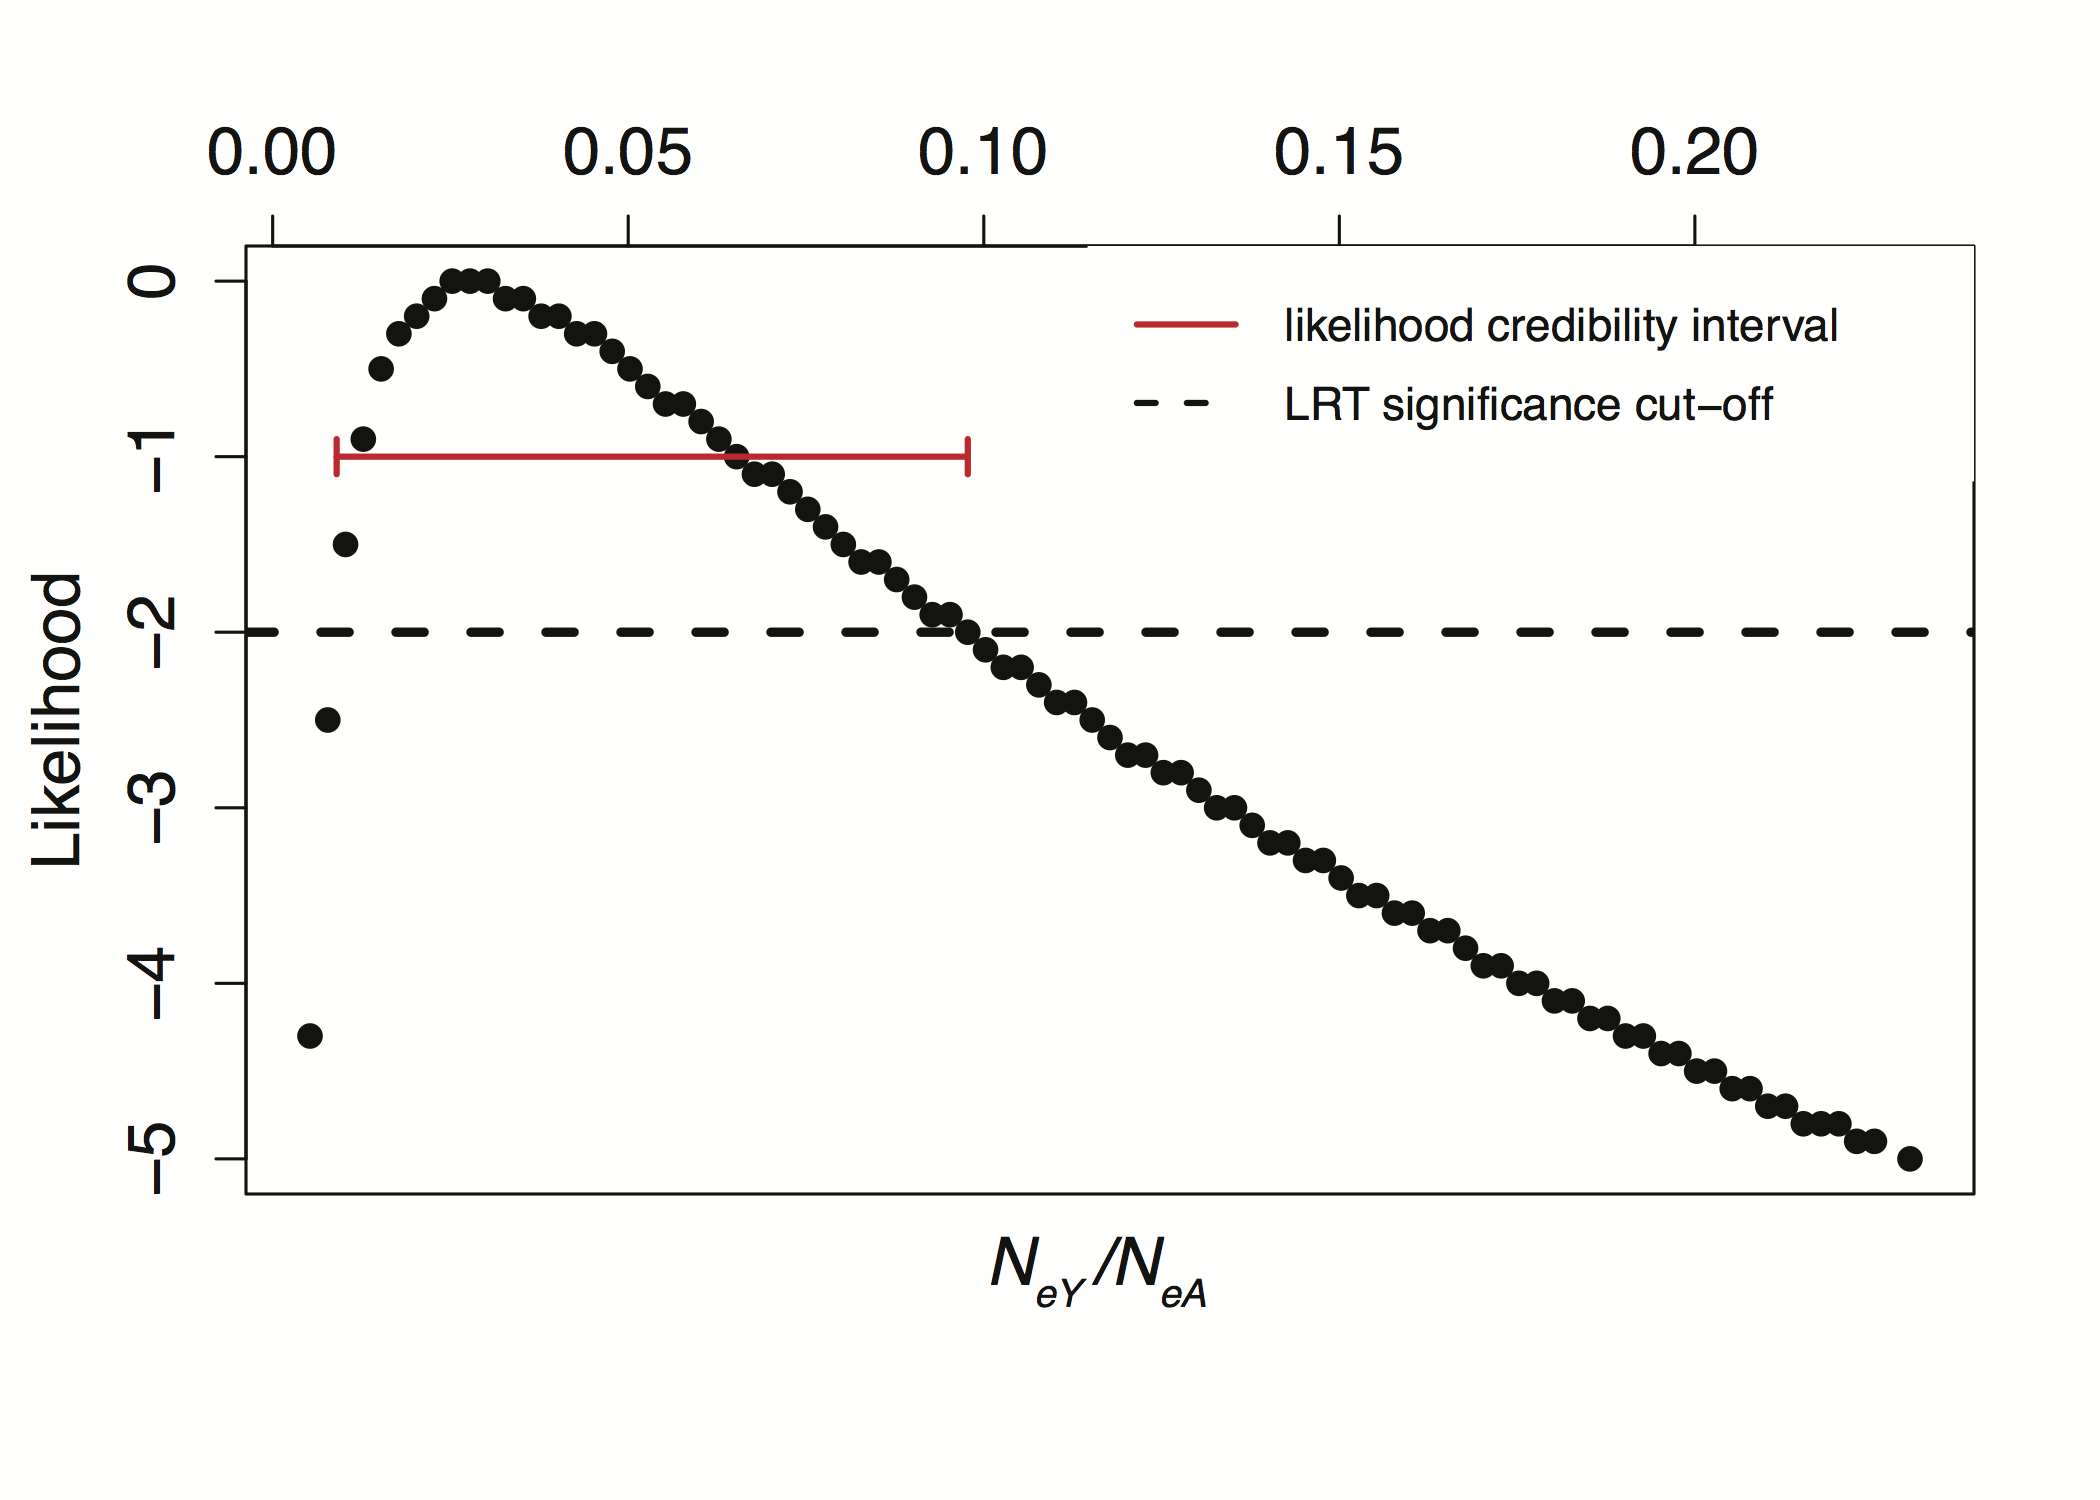
\includegraphics[width=.5\linewidth]{mlhka_figureS1.png}
\caption{MLHKA likelihood estimation of Y/A ratio. Explain more.}
\label{figure:mlhka_figureS1}
\end{figure}

\section*{SI Datasets}

\end{document}